% !TeX root = ../bachlor-arbeit.tex
The resulting algorithm is generally able to reproduce spectra from stacks generated based on the database.
This is a good first test because we know these spectra are possible and if the algorithm could not reproduce them something would be wrong. However, the goal was not to reproduce known spectra but to be able to find design parameters for new ones. Here the evaluation has to be more nuanced. Yes, some new transmission spectra, such as Gauß peaks, dips and sinus functions, are possible and can be seen in Appendix \ref{sec:apdx_B}.
But, the first limitation becomes apparent and is illustrated in figure \ref{fig:al:sine}.
The algorithm can successfully reproduce the sine with a maximum transmission of $0.7$ but not the sine with a maximum transmission of 1.
In general, for all fits, the maximum transmission has to stay below $\approx 0.7$ to be approximated successfully. This can be understood by the ohmic losses in plasmonic metasurfaces. Another limitation can be seen in figure \ref{gauspeak}. Even when the target function is approximated successfully there might be additional unwanted features in the spectrum. 
\\

\indent
Interestingly, some targets that would be trivial for a human are very challenging for the algorithm. If a human was tasked to create the maximum possible transmission at all wavelengths, he or she would probably use zero thickness metasurfaces or metasurfaces which only consist of holes. When the algorithm is given a transmission spectrum that is one everywhere it gets confused to a point of predicting negative parameters (figure \ref{one}).
They are chosen despite being completely out of bounds and thus very negatively affecting the simplexes loss function through equation \eqref{eq:al:simlex_loss}.
However, even this behavior can be explained because there are no zero thickness or hole only metasurfaces in the database we cannot expect the simplex to know about them.
Additionally, the less reachable a task is, the higher is the total loss and the less important is the boundary term explaining the nonsensical negative parameters.

\begin{figure}[H]
\centering
\begin{subfigure}{.5\textwidth}
    \centering
    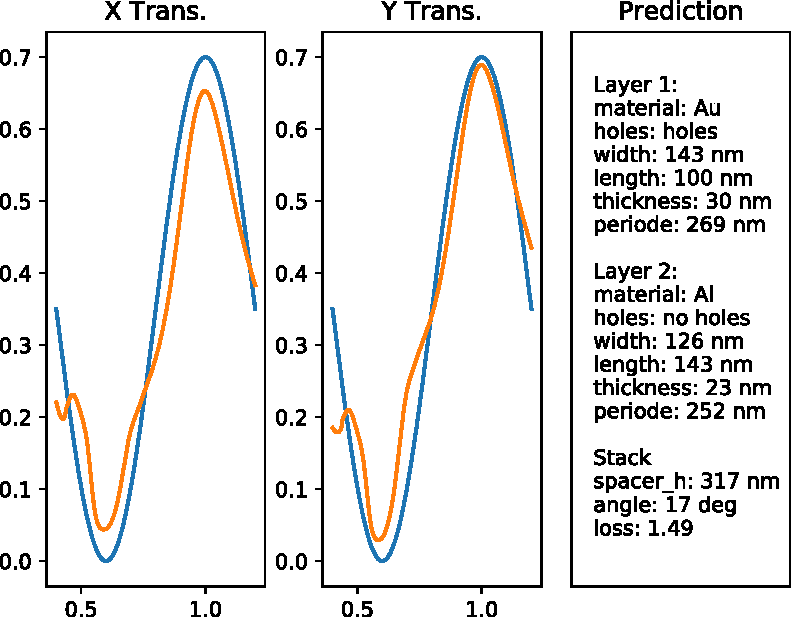
\includegraphics[width=.95\linewidth]{al_sine_07}
    \caption{}
    \label{fig:al:sine_succ}
\end{subfigure}%
\begin{subfigure}{.5\textwidth}
    \centering
    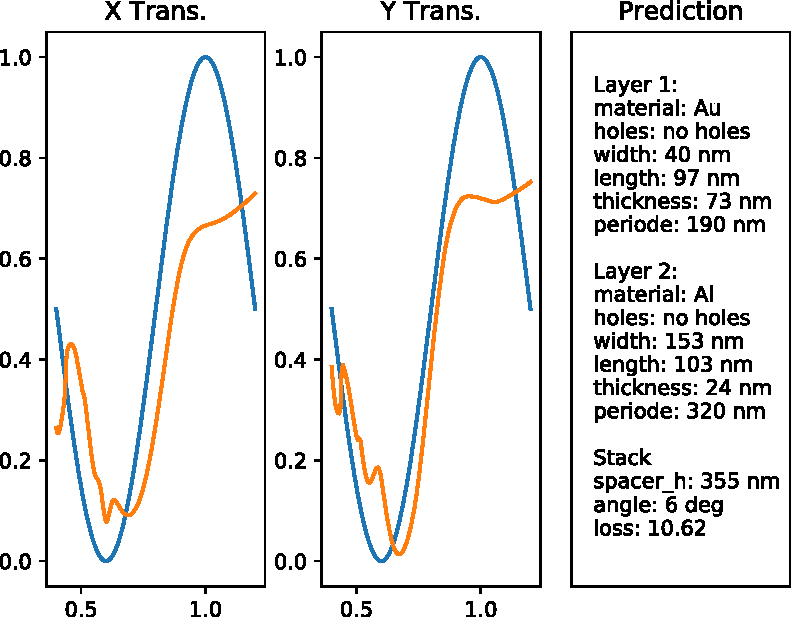
\includegraphics[width=.95\linewidth]{al_sine_fail}
    \caption{}
    \label{fig:al:sine_fail}
\end{subfigure}
\caption{Two fits of sine functions. Transmission in dependence of wave length. 0.4 to 1.2 $\mu$m. (a), the sine with a maximum transmission of $0.7$, could be reproduced successfully but (b), the sine with a maximum transmission of 1, could not.}
\label{fig:al:sine}
\end{figure}